   
        
        \begin{ledgroupsized}[r]{120mm}
        \footnotesize 
        \pstart        
        \noindent\textbf{\"{U}berlieferung:}  
        \pend
        \end{ledgroupsized}
      
       
              \begin{ledgroupsized}[r]{114mm}
              \footnotesize 
              \pstart \parindent -6mm
              \makebox[6mm][l]{\textit{L}}Konzept: LH XXXVIII Bl. 198\textendash 199. 1 Bog. 2\textsuperscript{o}. 2 1/2 S. zweispaltig. Bl. 199 r\textsuperscript{o} zur H\"{a}lfte beschrieben. Bl. 199 v\textsuperscript{o} leer. Zeichung auf Bl. 198 r\textsuperscript{o} in der unteren H\"{a}lfte rechts.\\KK 1, Nr. 1164 \pend
              \end{ledgroupsized}
        %\normalsize
        \vspace*{5mm}
        \begin{ledgroup}
        \footnotesize 
        \pstart
      \noindent\footnotesize{\textbf{Datierungsgr\"{u}nde}: Grundlage f\"{u}r die Datierung des St\"{u}ckes ist das Wasserzeichen, das f\"{u}r die 2. H\"{a}lfte 1671 gut nachgewiesen ist und sich auch noch am Beginn des Jahres 1672 findet.}
        \pend
        \end{ledgroup}
      
        \vspace*{8mm}
        \pstart 
        \normalsize
      [198 r\textsuperscript{o}] Quoniam in machina mea aer per \edtext{leve}{\lemma{}\Afootnote{leve \textbar\ tantum \textit{ gestr.}\ \textbar\ attrahitur: \textit{ L}}} attrahitur: et quovis momento tantum \edtext{aeris}{\lemma{}\Afootnote{aeris \textit{ erg.} \textit{ L}}} quantum fistula capit, \edtext{cujus}{\lemma{capit,}\Afootnote{ \textit{ (1) }\ quod \textit{ (2) }\ cujus \textit{ L}}} \edtext{aeris}{\lemma{}\Afootnote{aeris \textit{ erg.} \textit{ L}}} pondus quantumcunque sit, potentia \edtext{certe}{\lemma{}\Afootnote{certe \textit{ erg.} \textit{ L}}} levis minus est, et constat aerem nulla prorsus difficultate attrahi, modo aditus satis amplius ei pateat, praesertim cum ipse proprio nisu lubens irrumpat: Ideo arbitror leve \edtext{in aqua}{\lemma{leve}\Afootnote{ \textit{ (1) }\ 100 \textit{ (2) }\ in aqua \textit{ L}}} librae potentia implere aere posse follem qui capiat centum libras aquae et amplius. Neque enim aerem intra aquam leve retinet, sed fulcrum durum solidum, quod \edtext{aquae}{\lemma{quod}\Afootnote{ \textit{ (1) }\ aeris \textit{ (2) }\  aquae \textit{ L}}} nisum in aerem \edtext{ejiciendum, excipit}{\lemma{ejiciendum,}\Afootnote{ \textit{ (1) }\ aeris \textit{ (2) }\ excipit \textit{ L}}}; totumque follem sustinet. Leve ergo ipsum cum sustentaculo careat surget aeremque non resistentem attrahet, nec aqua aerem ejicere conans ipsi, sed toti renitetur. Hoc posito: \textso{unius librae vi procurari potest potentia 100 imo 1000 librarum}.\footnote{\textit{In H\"{o}he dieses Satzes rechts neben dem Text}: ist kein puppen-werck} Nec opus erit machinamento aliquo extra follem. Nam sufficit duo folli imminere alterum grave, alterum leve, \edtext{sed}{\lemma{leve,}\Afootnote{ \textit{ (1) }\ sed \textit{ (2) }\ aequalis ponderis \textit{ (3) }\ sed \textit{ L}}} vicissim, ita scilicet ut levi assurgente et follem diducente grave quiescat \edtext{prope fundum}{\lemma{quiescat}\Afootnote{ \textit{ (1) }\ in fu \textit{ (2) }\ prope fundum \textit{ L}}} follis seu basin nec diducenti obstet. Follis autem tanta vi assurgens deturbabit leve in locum infimum, ubi aliquandiu pendere cogetur, et attollet grave in operculum, quod rursus comprimet follem, eoque compresso iterum in basin labetur ibique quiescet, liberato levi, ut rursus ascendere in operculum, non tamen diducere possit, donec \edtext{totus}{\lemma{donec}\Afootnote{ \textit{ (1) }\ corpus \textit{ (2) }\ totus \textit{ L}}} follis descenderit quantum volumus. \pend
         \begin{center}
         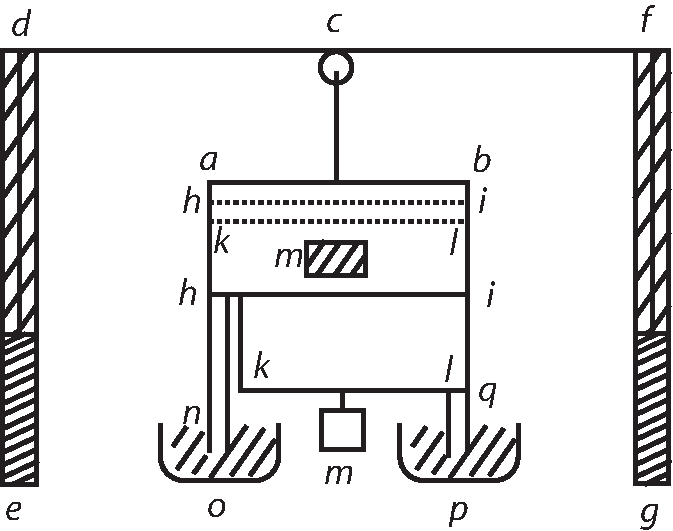
\includegraphics[width=0.55\textwidth]{images/38_198r}
         \\ \textit{[Fig. 1]} \\
         \end{center}
      \pstart Caeterum \edtext{quanquam}{\lemma{Caeterum}\Afootnote{ \textit{ (1) }\ quoniam \textit{ (2) }\ quanquam \textit{ L}}} machinamento follium multiplicatorum ita opus non est, \edtext{praebet tamen alium usum}{\lemma{est,}\Afootnote{ \textit{ (1) }\ pergendum tamen videtur \textit{ (2) }\ praebet tamen alium usum \textit{ L}}} deditque mihi occasionem cogitandi, an non \edtext{idem in libero aere solis siphonibus}{\lemma{idem}\Afootnote{ \textit{ (1) }\ solis s \textit{ (2) }\ in libero aere solis siphonibus \textit{ L}}} aquae immersis praestari possit. Quare est \edtext{follis sustentatus}{\lemma{follis}\Afootnote{ \textit{ (1) }\ grandis \textit{ (2) }\ quadratus \textit{ (3) }\ sustentatus \textit{ L}}}
      columnis, aut suspensus ex loco columnis \textit{de}, \textit{fg} sustenato divisus \edtext{si diducatur}{\lemma{}\Afootnote{si diducatur \textit{ erg.} \textit{ L}}} in regiones seu folles particulares quos hic non nisi duos repraesentabimus, \textit{abhi}, \textit{hikl}. Imae follis Tabulae \edtext{\textit{kl}}{\lemma{}\Afootnote{\textit{kl} \textit{ erg.} \textit{ L}}} appensum esto pondus \textit{m}. Cogitetur primum \edtext{totus}{\lemma{}\Afootnote{totus \textit{ erg.} \textit{ L}}} follis complicatus in eo situ quo tabulae \textit{hi}, \textit{kl} conspiciuntur punctatae. Ex regione superiore \edtext{\textit{abhi}}{\lemma{}\Afootnote{\textit{abhi} \textit{ erg.} \textit{ L}}} descendat siphon\protect\index{Sachverzeichnis}{siphon} \textit{hn} usque in interiora vasis aqua pleni \textit{o} ita tamen ut \edtext{fundum}{\lemma{ut}\Afootnote{ \textit{ (1) }\ inferiora \textit{ (2) }\ fundum \textit{ L}}} non attingat.\footnote{\textit{In der rechten unteren Ecke des Blattes}: Vereor ne quid isti machinamento obstet, nam simul laborantibus omnibus, non tamen singula totum assequentur, sunt enim singula viribus inaequalia ei quod trahunt, nec proinde sursum trahent, sed tantum in parte tantesimam, quot sunt divisiones. Est ergo hic Paralogismus valde speciosus vincent, sed non sursum trahent. Ruente ergo fundamento ruunt caetera omnia. Est tamen etiam ipsius non successus experimentum elegans.} Eodem \edtext{modo}{\lemma{}\Afootnote{modo \textit{ erg.} \textit{ L }%\hspace{10mm} 23 \hspace{3mm} trahunt, \textit{ (1) }\ quod \textit{ (2) }\ nec \textit{ L }\ \hspace{10mm} 24 \hspace{3mm} sunt \textbar\ sub \textit{ gestr.}\ \textbar\ divisiones. \textit{ L}%verschoben nach 198v%
      }} ex regione inferiore \textit{hikl} siphon\protect\index{Sachverzeichnis}{siphon} \textit{lq} in vas \textit{p} laxetur follis, sed ita ut primum aperiatur suprema regio, Folle igitur pondere diducto quantum fieri potest, ascendet aqua in siphonem\protect\index{Sachverzeichnis}{siphon} \textit{hn} quanta aequivalet ponderi \textit{m}. Pondus \textit{m} cum nihil amplius 